\section{Results}\label{sec:results}
\paragraph{Locked comparison.} Table~\ref{tab:primary} shows the original held-out primary experiment. The three individual channels retrieve 636, 635 and 635 designated references; equal-weight fusion raises this to 739/781. The pre-specified $k=3$ calibration obtains 749/781, a 1.28-percentage-point increase (14 newly correct, four regressions). Its exact McNemar $p=0.0309$ and the document-family bootstrap 95\% percentile interval $[+0.12,+2.44]$ percentage points indicate a positive \emph{within-benchmark} contrast under the stated assumptions. Ten test families improve, eight are unchanged and two decline. This is 10 fewer errors out of the baseline's 42.

\begin{table}[t]
\centering\small
\caption{Strict silver-reference R@1 on the identical BA48 781-query/780-candidate pool. IBM1 was added post-hoc and trained on 55,324 historical pairs; the starred $k=3$ contrast is the \emph{only} confirmatory test.}
\label{tab:primary}
\begin{tabular}{lrr}
\toprule
System & Correct & R@1 (\%) \\
\midrule
Dice (locked) & 636 & 81.43 \\
Character TF--IDF (locked) & 635 & 81.31 \\
E1 neural (locked) & 635 & 81.31 \\
Fusion (locked) & 739 & 94.62 \\
\textbf{Fusion + train $k=3$*} & \textbf{749} & \textbf{95.90} \\
\midrule
IBM1 symmetric (post-hoc) & 405 & 51.86 \\
IBM1 forward (post-hoc) & 294 & 37.64 \\
\bottomrule
\end{tabular}
\end{table}

\paragraph{Retrospective IBM1 reference.} We reproduced the public Nguyen et al.~\cite{nguyen2026parallelretrieval} implementation's \emph{development-selected hyperparameter profile}, but re-fitted both IBM1 directions on the historical 55,324 pairs: five EM passes, lowercase, accent and punctuation removal, smoothing $10^{-9}$ and length penalty 0.1. The symmetric score averages forward/backward lexical log-coverage. It achieves 405/781 (51.86\%) versus fusion's 739/781, while solving nine of the 32 silver-reference errors remaining after the locked $k=3$ correction. Training sources differ from the cited paper's 46,736-pair training split, so this is a \emph{within-BA48 baseline}, not a replication of its reported accuracy or evidence that adding IBM1 to fusion would help. R@5, R@10 and full-pool MRR are in Appendix~\ref{app:ibm1}.

\paragraph{Exploratory alternatives.} Table~\ref{tab:grid} lists the train-derived correction for several $k$ and Inverted Softmax (validation results are in Section~\ref{sec:robust}) with training-reference columns for several $\beta$; all rows except $k=3$ and $k=5$ were examined after test access, and the $p$-values are not adjusted for multiplicity. The $k=3$ rule is therefore \emph{not} the best observed normalization: train-derived Inverted Softmax at $\beta=2$ reaches 759/781 (97.18\%) with 20 corrections and no regression, yet its accuracy is peaked ($\beta=0.5$: 744, $\beta=1$: 750, $\beta=5$: 741, $\beta=10$: 735). Transductive Sinkhorn at $\beta=5$ reaches 770/781 (98.59\%) on the complete 781-query batch, with incomplete provenance for the original marginal specification (Section~\ref{sec:diagnostics}).

\begin{table}[t]
\centering\small
\caption{Train-derived normalizations on the 781-query test set (strict silver R@1; R@5 and MRR over the full 780-candidate pool). +/$-$: queries newly correct/newly wrong relative to fusion. Only $k=3$ (primary) and $k=5$ (sensitivity) were pre-specified.}
\label{tab:grid}
\begin{tabular}{lrrrrr}
\toprule
Method & R@1 & +/$-$ & exact $p$ & R@5 & MRR \\
\midrule
Fusion (locked) & 739 & -- & -- & 762 & .9600 \\
Train $k=1$ & 752 & +16/$-$3 & .004 & 766 & .9716 \\
Train $k=3$ (primary) & 749 & +14/$-$4 & .031 & 766 & .9690 \\
Train $k=5$ & 750 & +13/$-$2 & .007 & 766 & .9696 \\
Train $k=10$ & 752 & +14/$-$1 & .001 & 766 & .9709 \\
Inv.\ Softmax $\beta=1$ & 750 & +13/$-$2 & .007 & 767 & .9709 \\
Inv.\ Softmax $\beta=2$ & 759 & +20/$-$0 & $<$.001 & 769 & .9774 \\
Inv.\ Softmax $\beta=5$ & 741 & +19/$-$17 & .868 & 765 & .9625 \\
\bottomrule
\end{tabular}
\end{table}

\paragraph{Selection.} Choosing $k$ and $\beta$ on the validation split alone (Section~\ref{sec:robust}) selects $k=10$ and $\beta=2$; applied once to the test they give 752/781 and 759/781. A post hoc check inside the test set agrees: selecting the best setting on one random half of the 20 families and scoring it on the other half (4,000 splits) yields a mean held-out R@1 of 97.1\% against 95.9\% for fixed $k=3$ and 94.6\% for the baseline, with $\beta=2$ chosen in 97\% of the selections.

\section{Batch Dependence and Interpretation}\label{sec:diagnostics}
\paragraph{Query-batch stress.} Post-hoc subsampling retains all 780 candidates while randomly selecting fractions of held-out queries (200 draws per partial fraction). At 10\% query coverage, reported Sinkhorn $\beta=5$ declines from 98.59\% full-batch to 94.67\%; Sinkhorn $\beta=2$ retains 95.88\% and train-derived $k=3$ remains near 95.90\%. Train-derived Inverted Softmax $\beta=2$ stays near 97.1--97.3\%. Thus sensitivity is \emph{method- and temperature-specific}, not a universal failure of transduction. These draws reuse the same test and do not create independent evaluation replications. Fig.~\ref{fig:subsample} shows the fractions and Appendix~\ref{app:explore} lists the means.

\begin{figure}[t]
\centering
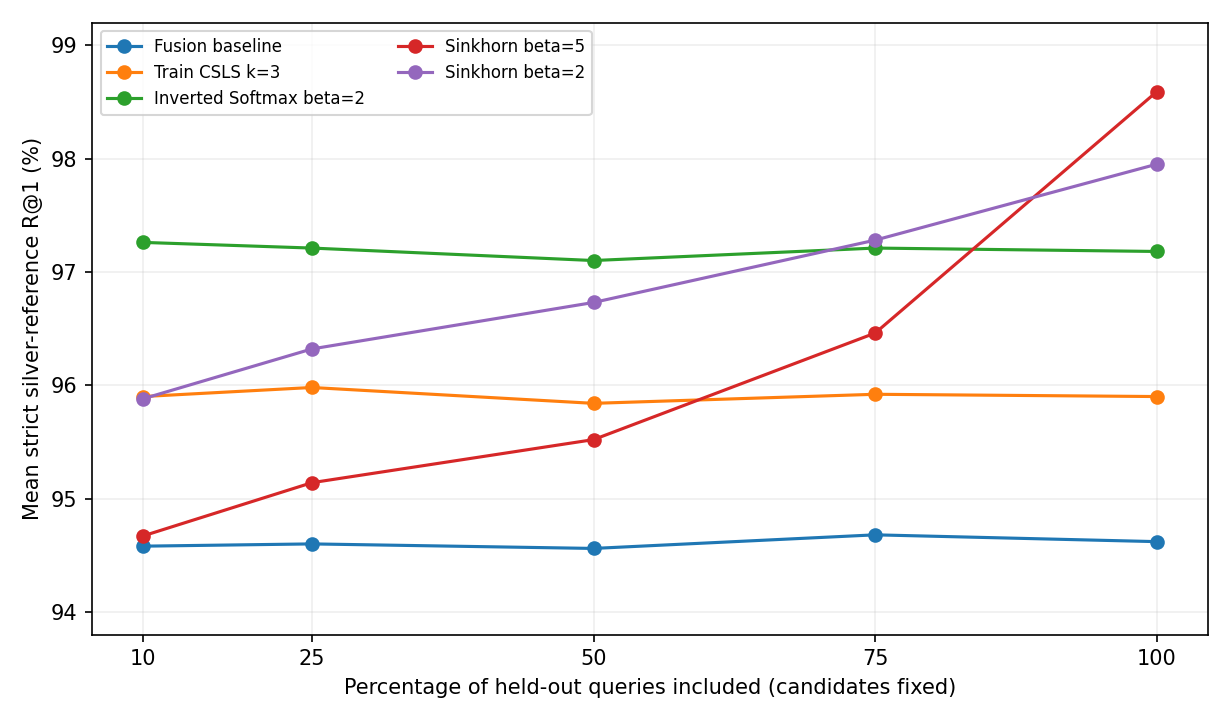
\includegraphics[width=0.85\textwidth]{query_subsampling.png}
\caption{Mean strict silver-reference R@1 as the fraction of held-out queries is reduced (candidates fixed at 780; 200 overlapping draws per partial fraction). The train-derived correction (k=3) is flat, whereas Sinkhorn at $\beta=5$ depends strongly on the batch.}
\label{fig:subsample}
\end{figure}

\paragraph{Mechanisms, not causal attribution.} Calibration makes top-1 assignments more evenly distributed (candidate-occupancy Gini 0.099 $\rightarrow$ 0.071), but the correlation between candidate density and the number of baseline top-1 errors assigned to a candidate is only about 0.02. This does not establish hubness as the source of all corrected errors. Since the neural component contributes in-sample E1 scores when estimating density from BA48 training queries, we also inspected retrospective out-of-fold E1$'$ controls. These use different encoders and improve their matched baselines but cannot substitute for a same-model out-of-fold experiment. No test in the present study adds genuinely unseen Vietnamese candidates, queries with no counterpart, or independent Bahnar-native source writing.
